\pagebreak
\chapter{Tuk Nextcloud}\label{sec:nextcloud}
Die Webanwendung \textit{Tuk Nextcloud} befindet sich unter der URL \url{http://tuk-nextcloud.auenland}. Zur Auflösung dieser URL wird der DNS-Server \textit{Auenland DNS} aus \autoref{sec:dns-auenland} benötigt. Alternativ kann auch die IP-Adresse \url{http://10.0.68.102} verwendet werden. Bei dieser Webanwendung handelt es sich um eine Nextcloud Cloud-Anwendung, bei der sich Nutzer über einen SSO-Provider anmelden und Daten mit dieser Cloud synchronisieren können. Die Webanwendung ist in \autoref{fig:04_nextcloud} dargestellt.

\vfill
\begin{figure}[!ht]
    \centering
    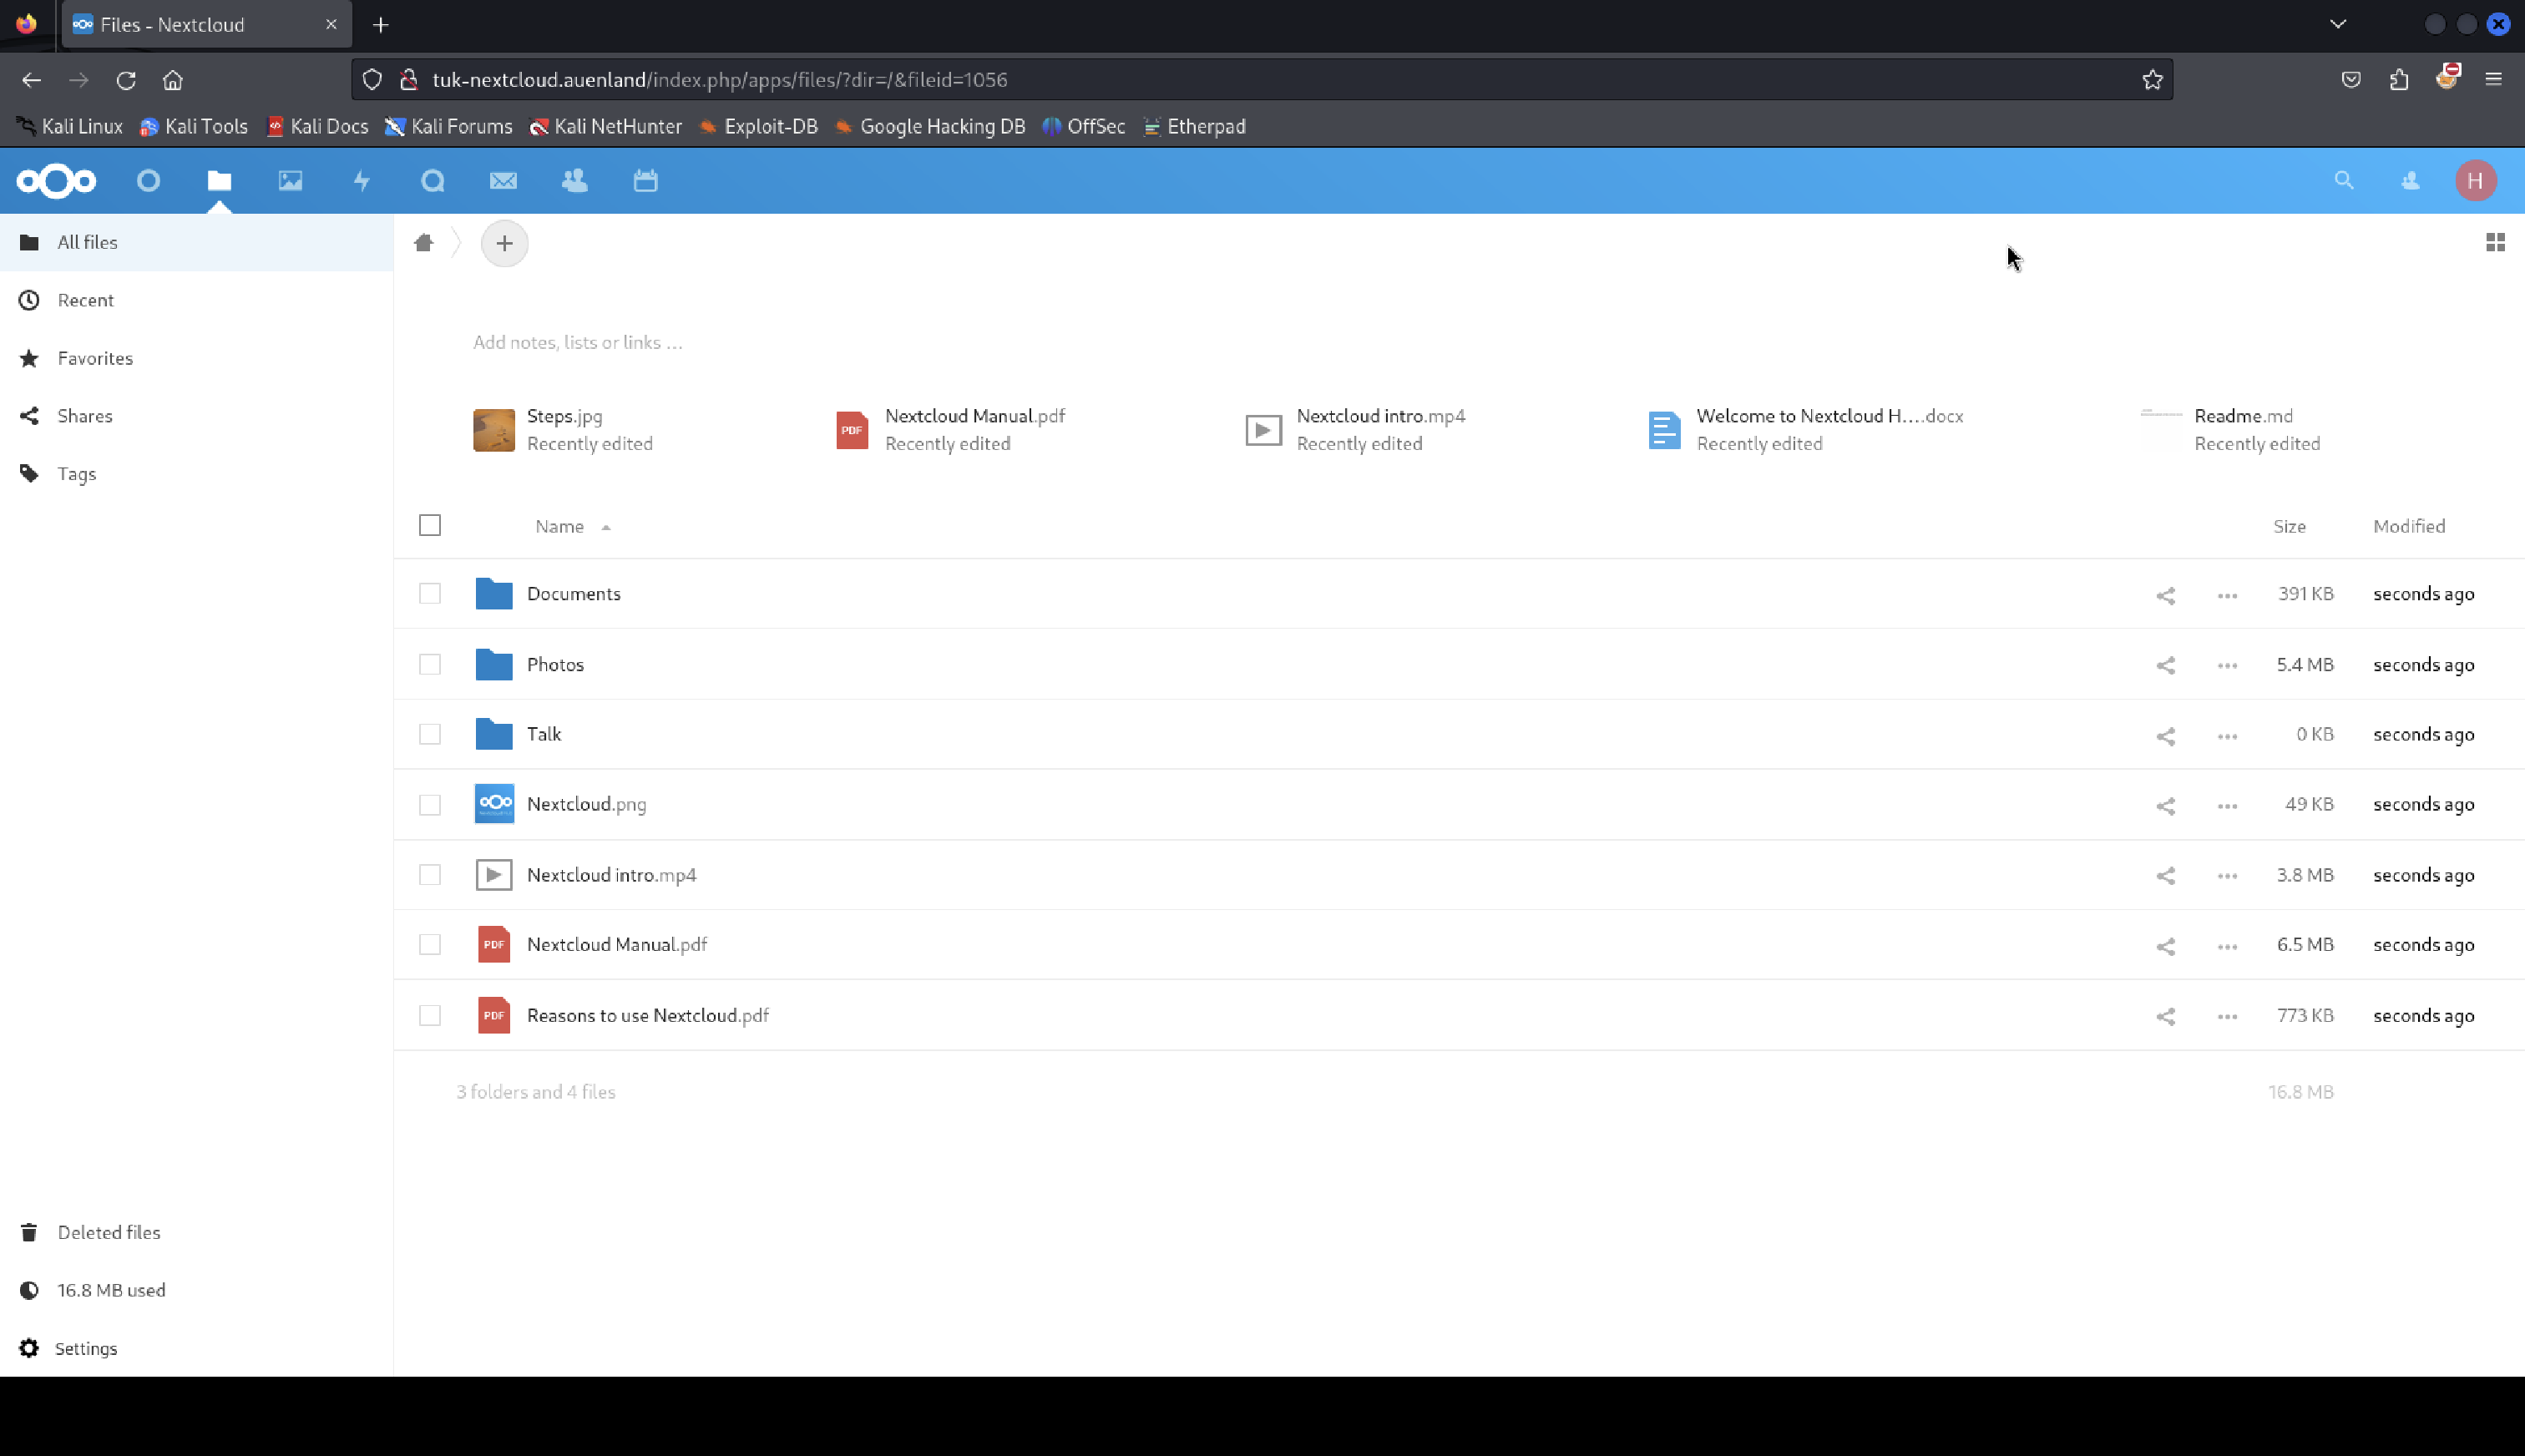
\includegraphics[width=\linewidth]{images/screenshots/06_nextcloud_2.png}
    \caption{Tuk Nextcloud Webanwendung}
    \label{fig:04_nextcloud}
\end{figure}
\vfill
\newpage

\cvss{av=local, ac=low, pr=none, ui=required, s=changed, c=low, i=low, a=low}
\cvssdescription{Schwache Authentifizierung ermöglicht Brute-Force-Angriff auf das Login-Formular. Zusätzlich erleichtert durch eine Dropdown-Liste mit den Benutzernamen.}

\section{\makecvssbadge Broken Authentication}
\cvssaddtosummary{Tuk Nextcloud: Broken Authentication}

\subsection*{Proof of concept}
Das Login-Formular der Webanwendung \textit{Tuk Nextcloud} gibt eine Dropdown-Liste mit Benutzernamen vor, was einen Brute-Force-Angriff auf diesen Login vereinfacht (siehe \autoref{fig:04_nextcloud_login}). Mit einem Tool wie der Burp Suite können solche Brute-Force-Angriffe durchgeführt werden. Mit einer Liste von Passwörtern und der Liste von Benutzernamen aus dem Dropdown-Menü wurde ein solcher Angriff durchgeführt. Dabei wurden drei gültige Zugangsdaten gefunden.\\

\begin{figure}[!ht]
    \centering
    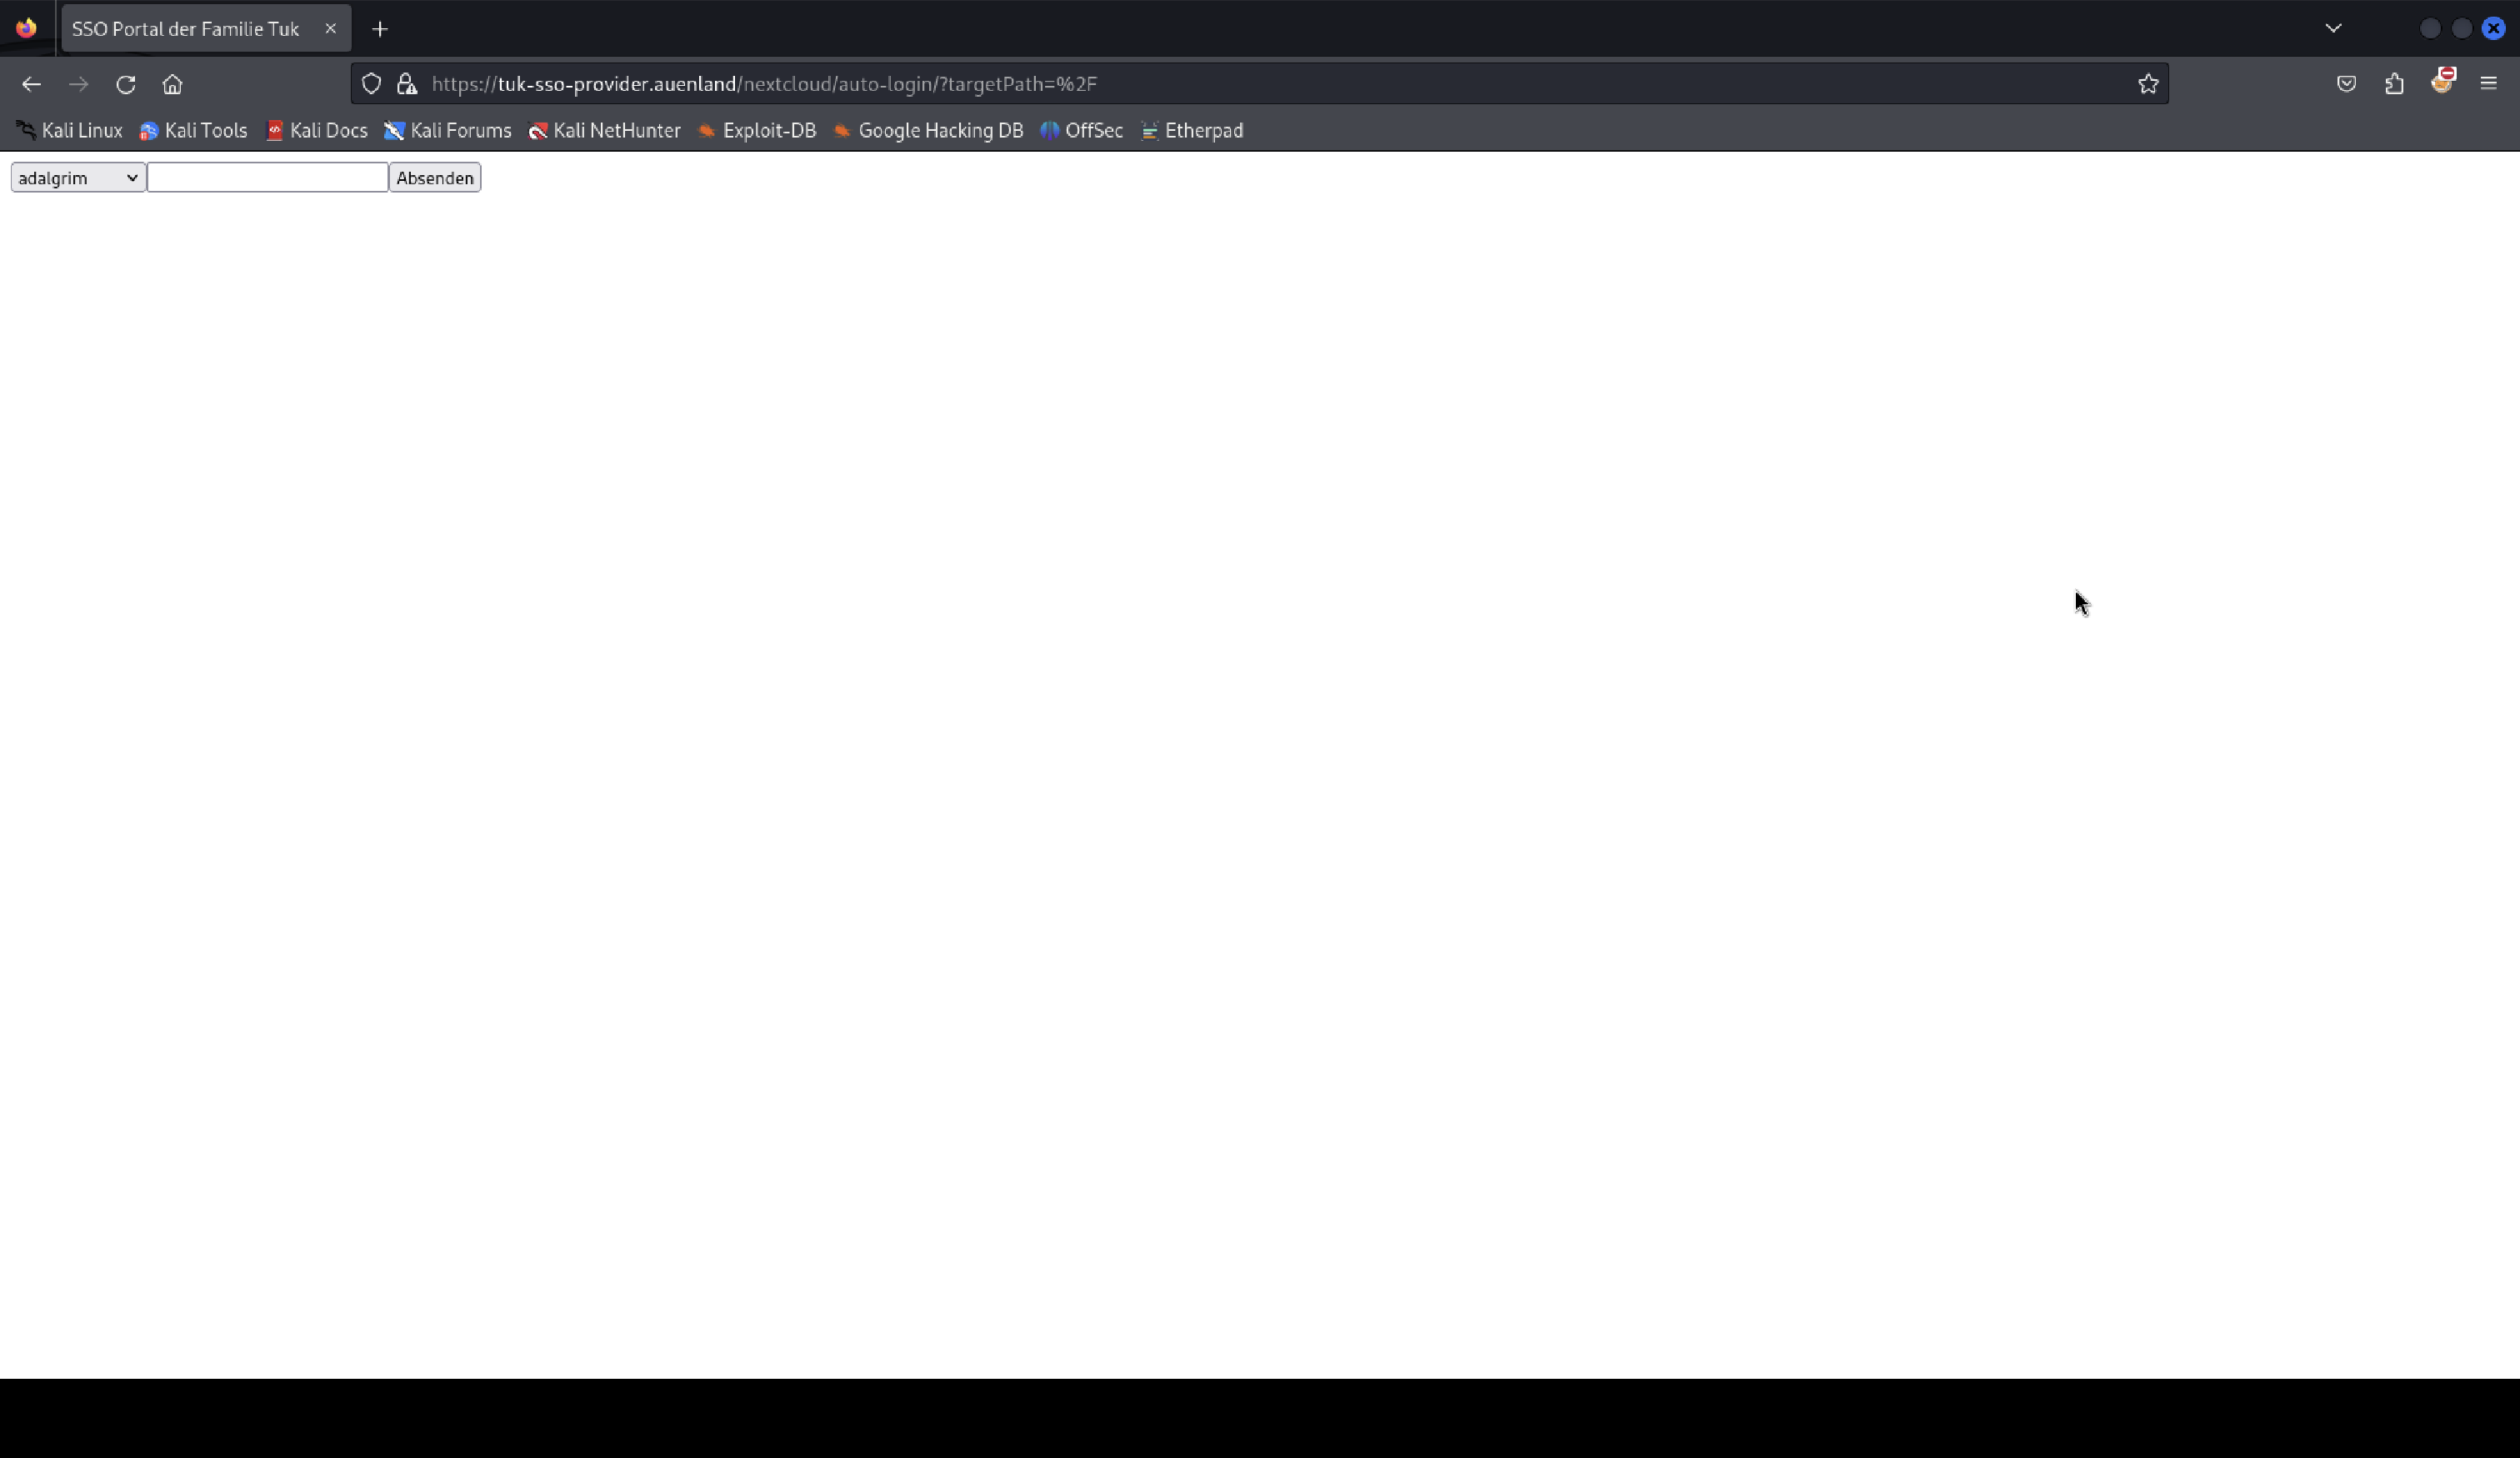
\includegraphics[width=\linewidth]{images/screenshots/06_nextcloud.png}
    \caption{Nextcloud-Webanwendung Login}
    \label{fig:04_nextcloud_login}
\end{figure}

\subsection*{Empfehlungen}
\begin{itemize}
    \item Benutzernamen nicht vorgeben: Benutzernamen sollten nicht als Drop-Down-Liste vorgegeben werden, da dies Angreifern die Durchführung von Brute-Force-Angriffen erleichtert.
    \item Strenge Passwortrichtlinien: Erzwingen Sie die Verwendung komplexer und langer Passwörter und ändern Sie Standardpasswörter, um einfache Passwörter zu vermeiden (siehe \cite{bsi_passwords}).
    \item Account-Sperrung und Ratenbegrenzung: Implementieren Sie Mechanismen, die nach mehreren fehlgeschlagenen Anmeldeversuchen eine Sperrung oder Verzögerung auslösen, um automatisierte Angriffe zu verhindern (siehe \cite{owaspAuthenticationOWASP}).
    \item Multi-Faktor-Authentifizierung (MFA): Ergänzt die Passwortauthentifizierung um einen zusätzlichen Faktor, um den Zugriff auch mit kompromittierten Zugangsdaten zu verhindern (siehe \cite{owaspAuthenticationOWASP}).
\end{itemize}

\cvss{av=local, ac=low, pr=none, ui=required, s=changed, c=low, i=low, a=low}
\cvssdescription{Aktiviertes Directory Listing und schwache Zugriffrechte erlauben es Nutzern sämtliche Serverdateien zu durchsuchen.}

\section{\makecvssbadge Sensitive Data Exposure}
\cvssaddtosummary{Tuk Nextcloud: Sensitive Data Exposure} 

\subsection*{Proof of concept}
Nachdem die Zugangsdaten mehrere Nutzer erlangt wurden, kann sich mit einem dieser in die Webanwendung einloggt werden. Nach erfolgreicher Authentifizierung erlaubt das aktivierte Directory Listing in Kombination mit unzureichend eingeschränkten Zugriffsrechten auf die Serverdateien, dass sämtliche Dateien auf dem Webserver durchsucht werden können. Im Verzeichnis \texttt{/data/pippin/files/} wurden mehrere Versionen der Datei \texttt{Passwords.kdbx} festgestellt.

\subsection*{Empfehlungen}
\begin{itemize}
    \item Deaktivierung des Directory Listings: Deaktivieren Sie das Directory Listing, damit die Inhalte von Verzeichnissen nicht aufgelistet werden (siehe \cite{owaspSecurityMisconfiguration}).
    \item Einschränkung der Zugriffsrechte: Schränken Sie die Zugriffsrechte aller Dateien so ein, das die ordungsgemäße Nutzung gegeben ist, aber auch nur die nötigsten Zugriffsrechte vergeben sind nach dem Least-Privilege-Prinzip (siehe \cite{owaspSecurityMisconfiguration}).
    \item Sichere Verschlüsselung sensibler Daten: Verschlüsseln Sie sensible Daten mit einem sicheren Verschlüsselungsalgorithmus und verwenden Sie sichere Passwörter zum Schützen von Dateien. Achten Sie außerdem darauf, dass ältere unsichere Datei-Versionen im Papierkorb vorhanden sind (siehe \cite{owaspSecurityMisconfiguration}).
\end{itemize}

\cvss{av=local, ac=low, pr=none, ui=required, s=changed, c=low, i=low, a=low}
\cvssdescription{Unsichere JWT-Implementierung führt dazu, dass valide JWT-Tokens für beliebige Nutzer generiert werden können.}

\section{\makecvssbadge Unsichere JWT-Implementierung}
\cvssaddtosummary{Tuk Nextcloud: Unsichere JWT-Implementierung} 

\subsection*{Proof of concept}
Nach der Anmeldung mit einem der Benutzer kann der JWT-Token abgefangen werden, der nach erfolgreicher Authentifizierung gesendet wird. Dieser Token kann mit dem Tool John-The-Ripper gecrackt werden. Anschließend kann auf der Website \url{https://jwt.io} ein neuer gültiger JWT-Token für einen beliebigen Benutzer erstellt werden. 

\subsection*{Empfehlungen}
\begin{itemize}
    \item Sichere Token-Signierung: Verwenden Sie einen sicheren Algorithmus zum Signieren der Tokens. Zusätzlich können die Inhalte Verschlüsselt werden. Dadurch wird das cracken der Tokens deutlich erschwert (siehe \cite{owaspSessionManagement}).
    \item Kurze Token-Lebensdauer: Durch die Verwendung von kurzen Lebensdauern für JWT-Tokens, ist es schwerer für Angreifer die Tokens zu cracken (siehe \cite{owaspSessionManagement}).
    \item Sichere Übertragung: Werden die Tokens ausschließlich über eine sichere HTTPS Verbindung verschickt, können diese nur schwer abgefangen werden (siehe \cite{owaspSessionManagement}).
\end{itemize}

\cvss{av=network, ac=low, pr=none, ui=required, s=changed, c=high, i=high, a=high}
\cvssdescription{Über den Dateiupload der Nextcloud-Anwendung konnte eine Webshell hochgeladen werden, die durch aktiviertes Directory Listing und mangelnde Zugriffsbeschränkungen ausgeführt werden konnte.}

\section{\makecvssbadge Remote Code Execution (RCE)}
\cvssaddtosummary{Tuk Nextcloud: Remote Code Execution (RCE)} 

\subsection*{Proof of concept}
Mit einem der erhaltenen Benutzeraccounts kann sich erneut in die Webanwendung eingeloggt werden. Anschließend kann über den integrierten Dateiupload der Nextcloud-Anwendung eine PHP-Shell hochgeladen werden. Über das aktivierte Directory Listing kann das Dateiverzeichnis des Nutzers gefunden werden. In diesem Verzeichnis befindet sich die hochgeladene Webshell (z.B. unter \url{http://tuk-nextcloud.auenland/data/heiderose/files/webshell_password.php}). Wird diese URL geöffnet, öffnet sich die Webshell und es können Systemkommandos auf dem Web Server ausgeführt werden. 

Nun kann auf dem Angreifersystem ein Netcat-Listener mit dem Befehl aus \autoref{listing:netcat-listener} gestartet werden. Anschließend kann eine Reverse Shell über die hochgeladene Webshell mit dem Befehl aus \autoref{listing:bash-reverse-shell} gestartet werden. Ein Nachweis ist in \autoref{fig:04_nextcloud_proof} dargestellt.

\begin{figure}[!ht]
    \centering
    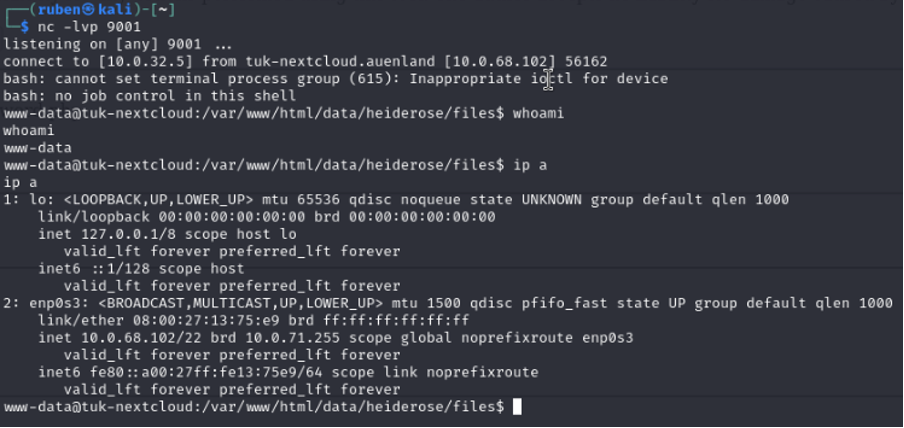
\includegraphics[width=\linewidth]{images/proofs/04_nextcloud_proof.png}
    \caption{Proof für die Nextcloud-Webanwendung}
    \label{fig:04_nextcloud_proof}
\end{figure}

\subsection*{Empfehlungen}
\begin{itemize}
    \item Sichere Dateiuploads: Upload-Verzeichnisse sollten so konfiguriert werden, dass darin hochgeladene Dateien nicht als PHP-Code ausgeführt werden können (z.B. durch entsprechende Serverkonfiguration oder mittels .htaccess-Regeln) (siehe \cite{owaspFileUpload}).
\end{itemize}

